\documentclass[final,hyperref={pdfpagelabels=false}]{beamer}
\usepackage{grffile}
\mode<presentation>{\usetheme{ECOMP}}
\usepackage[portuguese, brazil]{babel}   
\usepackage[utf8]{inputenc}
\usepackage{amsmath,amsthm, amssymb, latexsym}
%\usepackage{times}\usefonttheme{professionalfonts}  % obsolete
%\usefonttheme[onlymath]{serif}
\boldmath
\usepackage[orientation=portrait,size=a0,scale=1.4,debug]{beamerposter}
% change list indention level
% \setdefaultleftmargin{3em}{}{}{}{}{}


%\usepackage{snapshot} % will write a .dep file with all dependencies, allows for easy bundling

\usepackage{array,booktabs,tabularx}
\newcolumntype{Z}{>{\centering\arraybackslash}X} % centered tabularx columns
\newcommand{\pphantom}{\textcolor{ta3aluminium}} % phantom introduces a vertical space in p formatted table columns??!!

\listfiles

%%%%%%%%%%%%%%%%%%%%%%%%%%%%%%%%%%%%%%%%%%%%%%%%%%%%%%%%%%%%%%%%%%%%%%%%%%%%%%%%%%%%%%
\graphicspath{{figures/}}
 
\title{\huge Visualização de Dados de Informações Extraídas da Web - Um Estudo sobre Conteúdo Popular Japonês}
\author{Gabriel Fontenelle Senno Silva\inst{1}}
\institute[SENAC]{Centro Universitário Senac - Campus Santo Amaro}
\date[Dezembro 3th, 2014]{Dezembro 03, 2014}

%%%%%%%%%%%%%%%%%%%%%%%%%%%%%%%%%%%%%%%%%%%%%%%%%%%%%%%%%%%%%%%%%%%%%%%%
\newlength{\columnheight}
\setlength{\columnheight}{105cm}
%%%%%%%%%%%%%%%%%%%%%%%%%%%%%%%%%%%%%%%%%%%%%%%%%%%%%%%%%%%%%%%%%%%%%%%%
\begin{document}%Inicia o documento
\begin{frame}
  \begin{columns}%Inicia as Colunas
    % ---------------------------------------------------------%
    % Configurar a primeira coluna
\begin{column}{.49\textwidth}
      \begin{beamercolorbox}[center,wd=\textwidth]{postercolumn}
        \begin{minipage}[T]{.95\textwidth} % tweaks the width, makes a new \textwidth
          \parbox[t][\columnheight]{\textwidth}{ % must be some better way to set the the height, width and textwidth simultaneously
            % Since all columns are the same length, it is all nice and tidy.  You have to get the height empirically
            % ---------------------------------------------------------%
            % fill each column with content
            
            %%RESUMO%%%%%%%%%%%%%%%%%
            \begin{block}{Resumo}
            Este trabalho apresenta um estudo sobre conteúdo popular japonês por meio de visualizações geradas com dados extraídos automaticamente de websites com grande quantidade de dados. 
            \end{block}
            \vfill
            %%INTRODUÇÃO%%%%%%%%%%%%%
            \begin{block}{Introdução}
            Visualização de dados é a comunicação visual de informações, com base em um conjunto de dados. Crawler é um programa que navega automaticamente em websites e extraí dados de páginas determinadas.\\
            Este trabalho apresenta visualizações de dados, desenvolvidos a partir de dados extraídos de websites com o uso de sistema de \emph{crawling}. Foram escolhidos websites sobre conteúdo popular japonês. A cultura popular japonesa é conhecida pelo desenvolvimento de animações, revistas em quadrinhos e gêneros literários influenciados por um estilo de desenho único focado nas expressões de suas personagens. 
            \end{block}
            \vfill
            %%%%%%%%%%OBJETIVOS%%%%%%%%%%%%%%
            \begin{block}{Objetivo}
            Este trabalho apresenta um estudo sobre conteúdo popular japonês, exibindo informações com dois tipos de visualizações de dados: nuvem de palavras e nuvem de bolhas. As informações são obtidas a partir de dados extraidos com \emph{crawling} de websites definidos.  
            %Este trabalho tem por objetivo obter informações de franquias de conteúdo popular japonês e exibí-las na forma de visualização de duados. 
			%Para gerar as visualizações foi modelado o banco de dados e desenvolvido o sistema de crawling para extração de dados automaticamente de websites definidos. 
		
            \end{block}
        	\vfill   
            \begin{block}{Websites}
           Foram escolhidos pela popularidade e pela quantidade de itens que possuem os websites abaixo:
			\begin{itemize}
			\item http://www.mangaupdates.com/
			\item http://myfigurecollection.net/
			\item http://animecharactersdatabase.com/
			\end{itemize}
			
			Para armazenar os dados um extenso banco de dados foi modelado, antes que o sistema de \emph{crawling}, com a biblioteca Scrapy, pudesse ser utilizado. Durante a execução do crawler os dados foram normalizados e inseridos no banco de dados PostgreSQL. 
            \end{block}
            \vfill 
            %%%%%%%%%%%%%METODOLOGIA%%%%%%%%
            \begin{block}{Metodologia}
			Área ocupada por pixels pode ser cálculada rapidamente utilizando a estrutura de dados Imagem Integrada. Se a área calculada em determinado local for maior que zero ela está ocupada.
			Cada valor na Imagem Integral equivale ao resultado da soma de todos os elementos das linhas e das colunas anteriores de matriz utilizada em sua criação.
			\begin{figure}[H]
			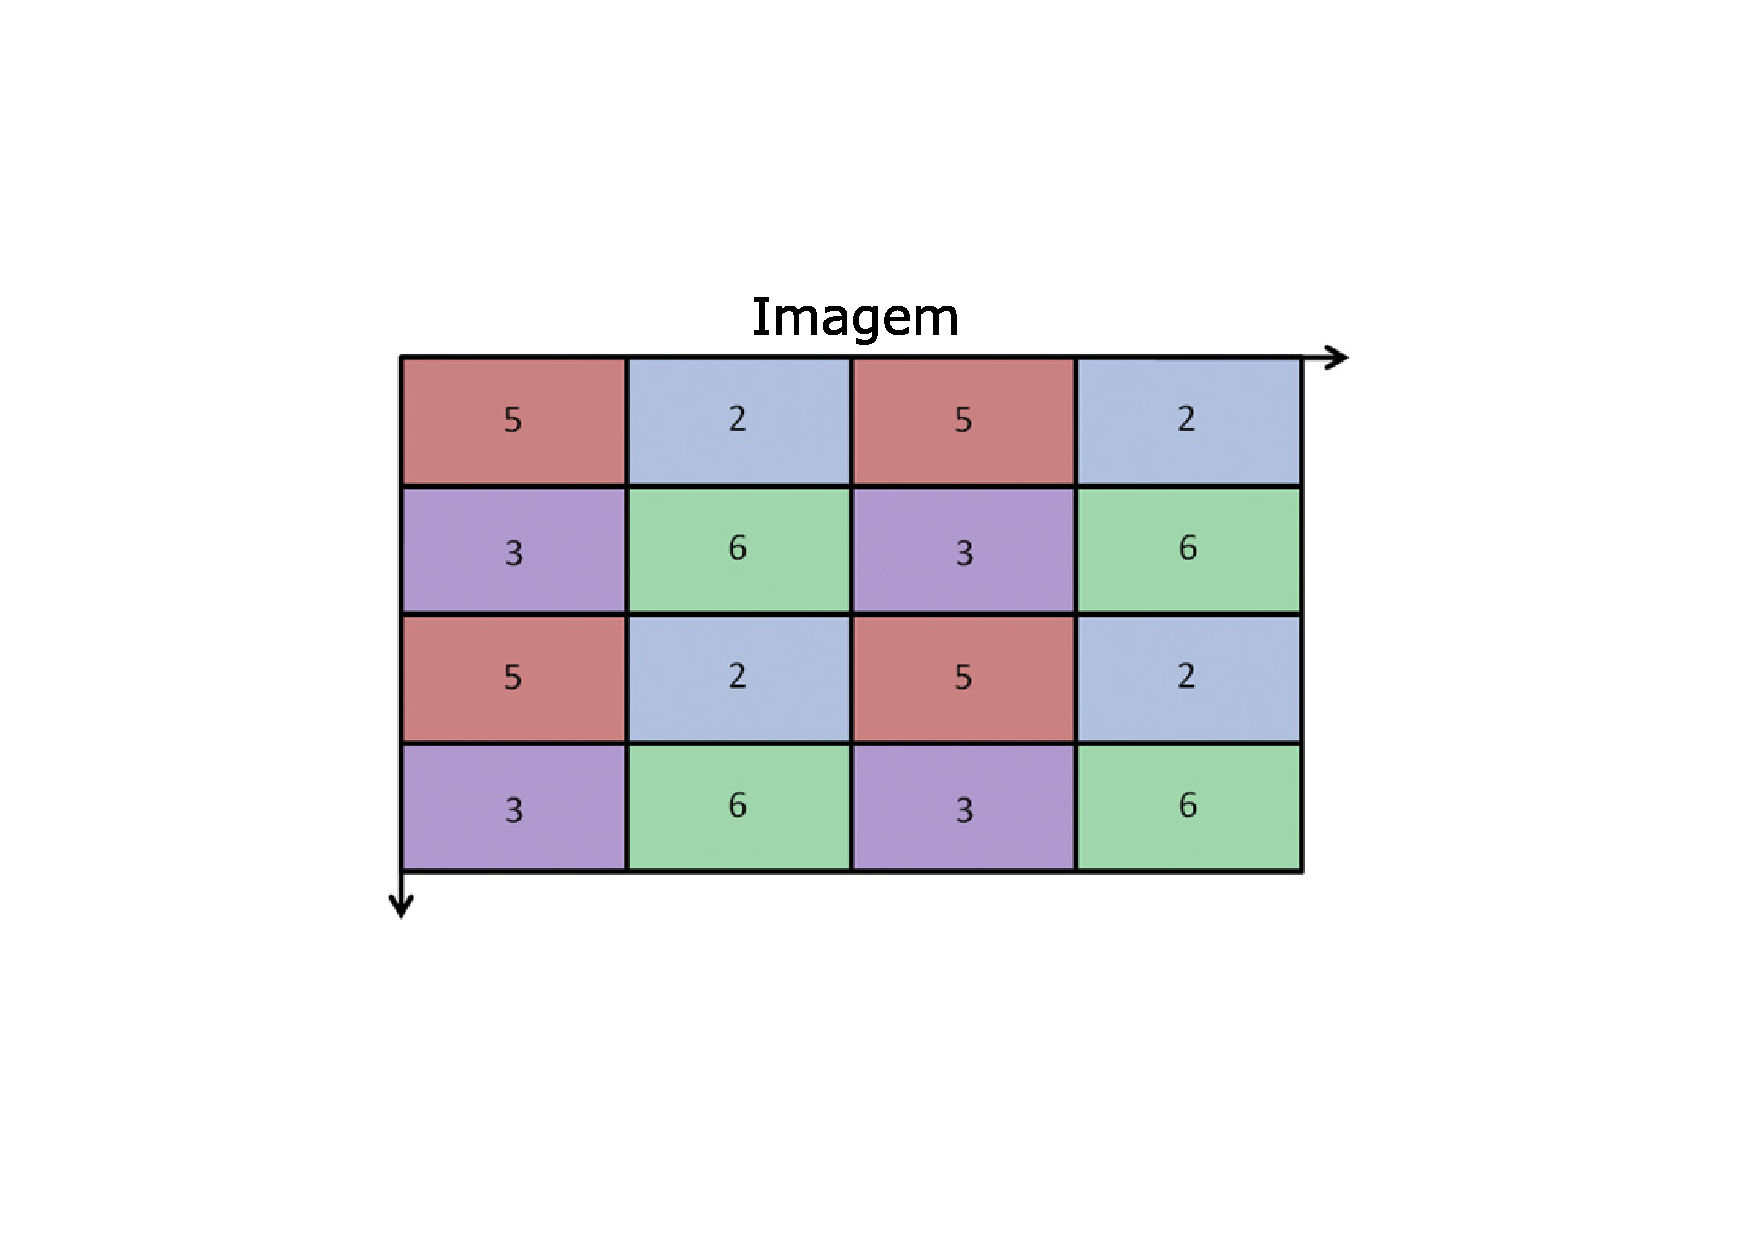
\includegraphics[width=0.35\linewidth]{image.pdf}
			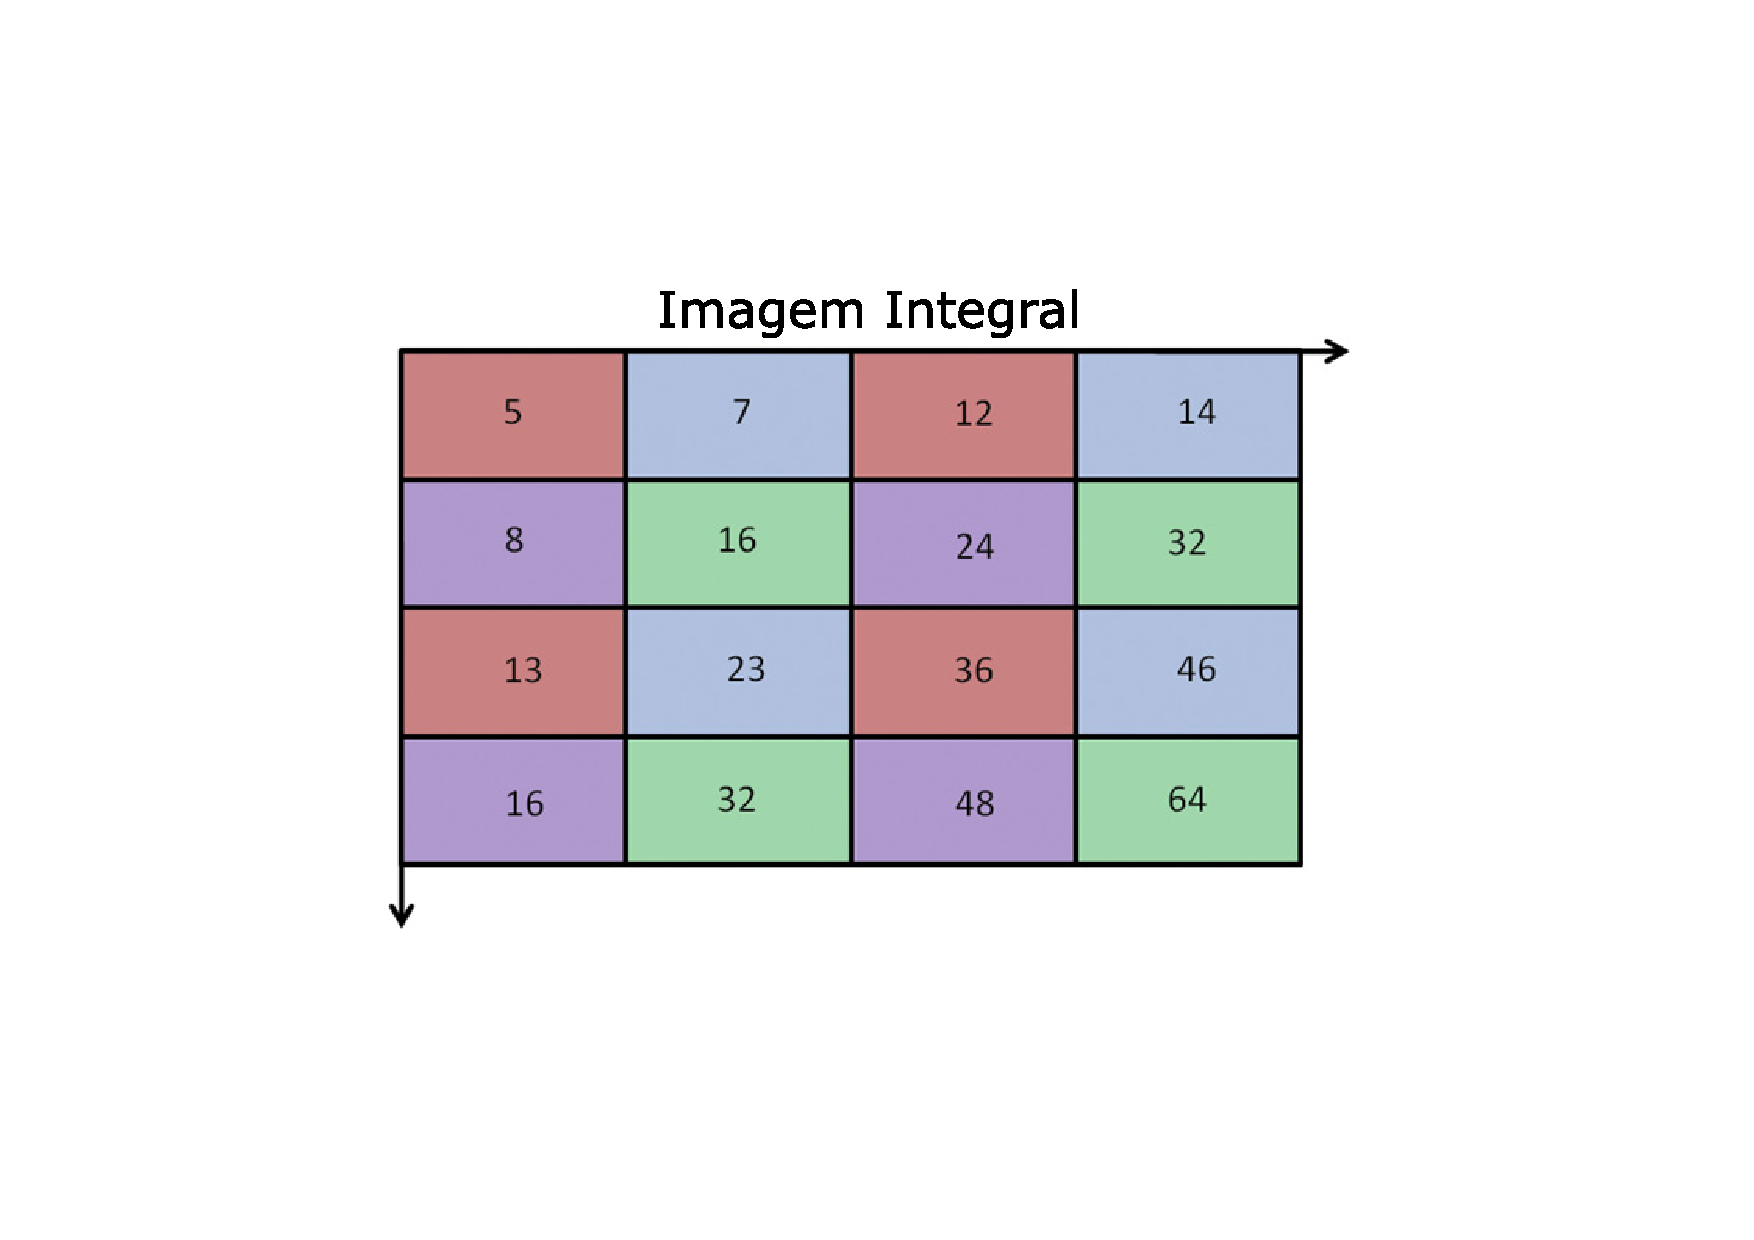
\includegraphics[width=0.35\linewidth]{integral.pdf} 
			\end{figure}
            Para calcular a área com a Imagem Integral se utiliza a seguinte fórmula:
            \begin{equation} 
            \acute{a}rea = I(i,j) + I(i + 1,j + 1) - I(i + 1,j) - I(i,j + 1).
            \end{equation}
            
            I representa a Imagem Integral e (i,j) representam as linhas e colunas.\\
            ~\\
            \textbf{Obtendo uma máscara}\\
			Como espaços disponívels são iguais a zero, utilizando uma imagem com ilustração na cor preta, por ter valor zero, pode ser obtida uma máscara que restringirá a posição de palavras ou círculos. A seguir exemplo de imagem máscara:
            \begin{figure}[H]
            
\includegraphics[width=0.35\linewidth]{e-comp-24502.pdf}
             \caption{Máscara usando a letra e de e-comp} \label{collaborator}
             \end{figure}
             
            \end{block}
            \vfill
          }
          % ---------------------------------------------------------%
          % end the column
        \end{minipage}
      \end{beamercolorbox}
    \end{column}
    % ---------------------------------------------------------%
    % Fim da coluna 1

    % ---------------------------------------------------------%
    % Ajuste da Coluna 2
    \begin{column}{.49\textwidth}
      \begin{beamercolorbox}[center,wd=\textwidth]{postercolumn}
        \begin{minipage}[T]{.95\textwidth} % tweaks the width, makes a new \textwidth
          \parbox[t][\columnheight]{\textwidth}{
          	\begin{block}{Metodologia}
            \textbf{Definindo o tamanho dos textos e dos círculos}\\
              \begin{equation} 
tamanho = \frac{c * ranking}{\ln(ranking + 10)}
\end{equation}

Onde:

\begin{itemize}  
  \item c é a razão entre a área útil da máscara e a quantidade de objetos a serem inseridos.
\end{itemize}
Para evitar divisão por zero é somado o valor 10 ao número \emph{ranking} antes do cálculo do Logaritmo Natural.\\
~\\
Com o tamanho definido dos objetos (textos ou círculos), verificamos na Imagem Integral da máscara os espaços disponíveis e determinamos uma posição entre eles. Adicionamos portanto o objeto a imagem máscara e geramos uma nova Imagem Integral. Repetimos esse procedimento para cada objeto retirado do banco de dados. E por fim salvamos uma imagem com todos os objetos posicionados. 
            \end{block}
            \vfill
            \begin{block}{Resultados: Nuvens de palavras e de bolhas}
            \begin{figure}[H]
            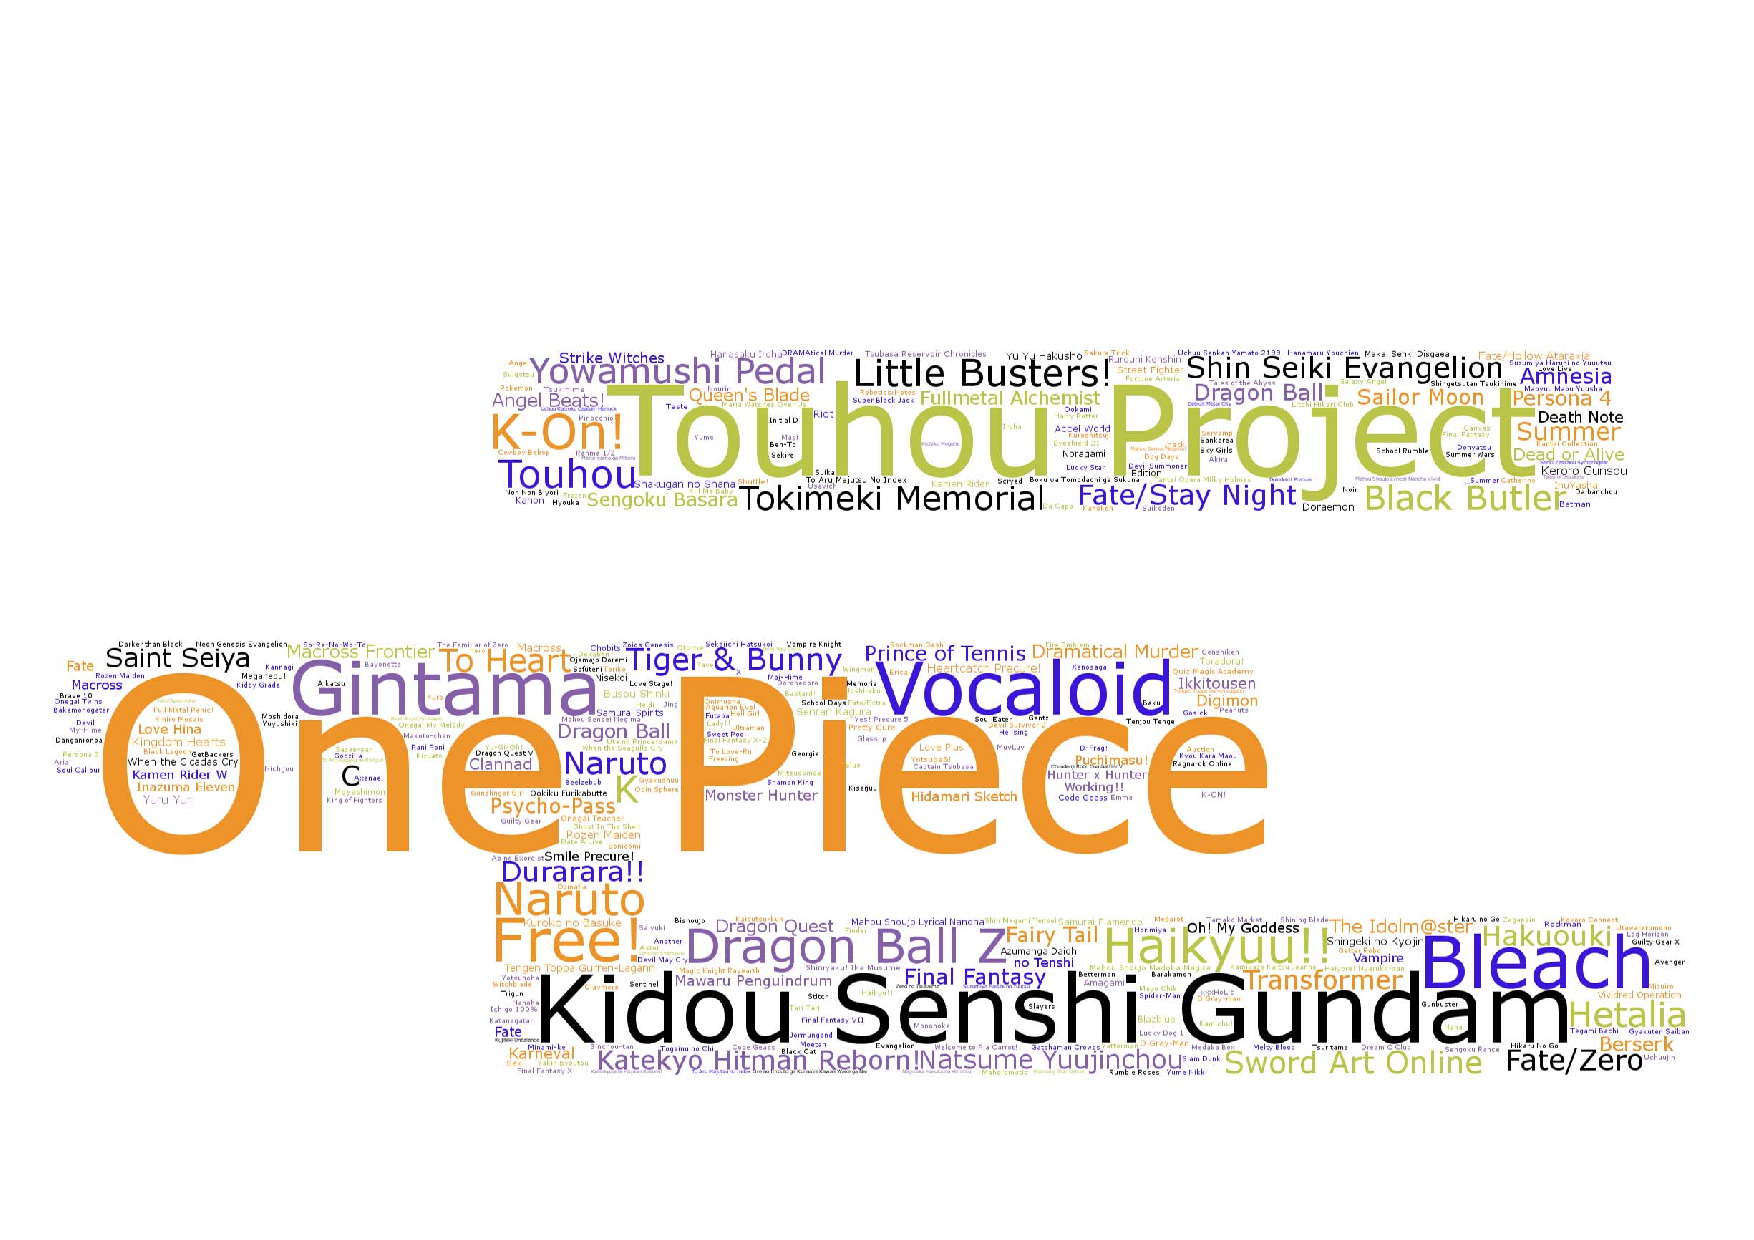
\includegraphics[width=0.8\linewidth]{Full_page_photo.pdf}
            \caption{Franquias com tamanho definido pela quantidade de itens que possuem} \label{collaborator}
             \end{figure}
             \begin{figure}[H]
             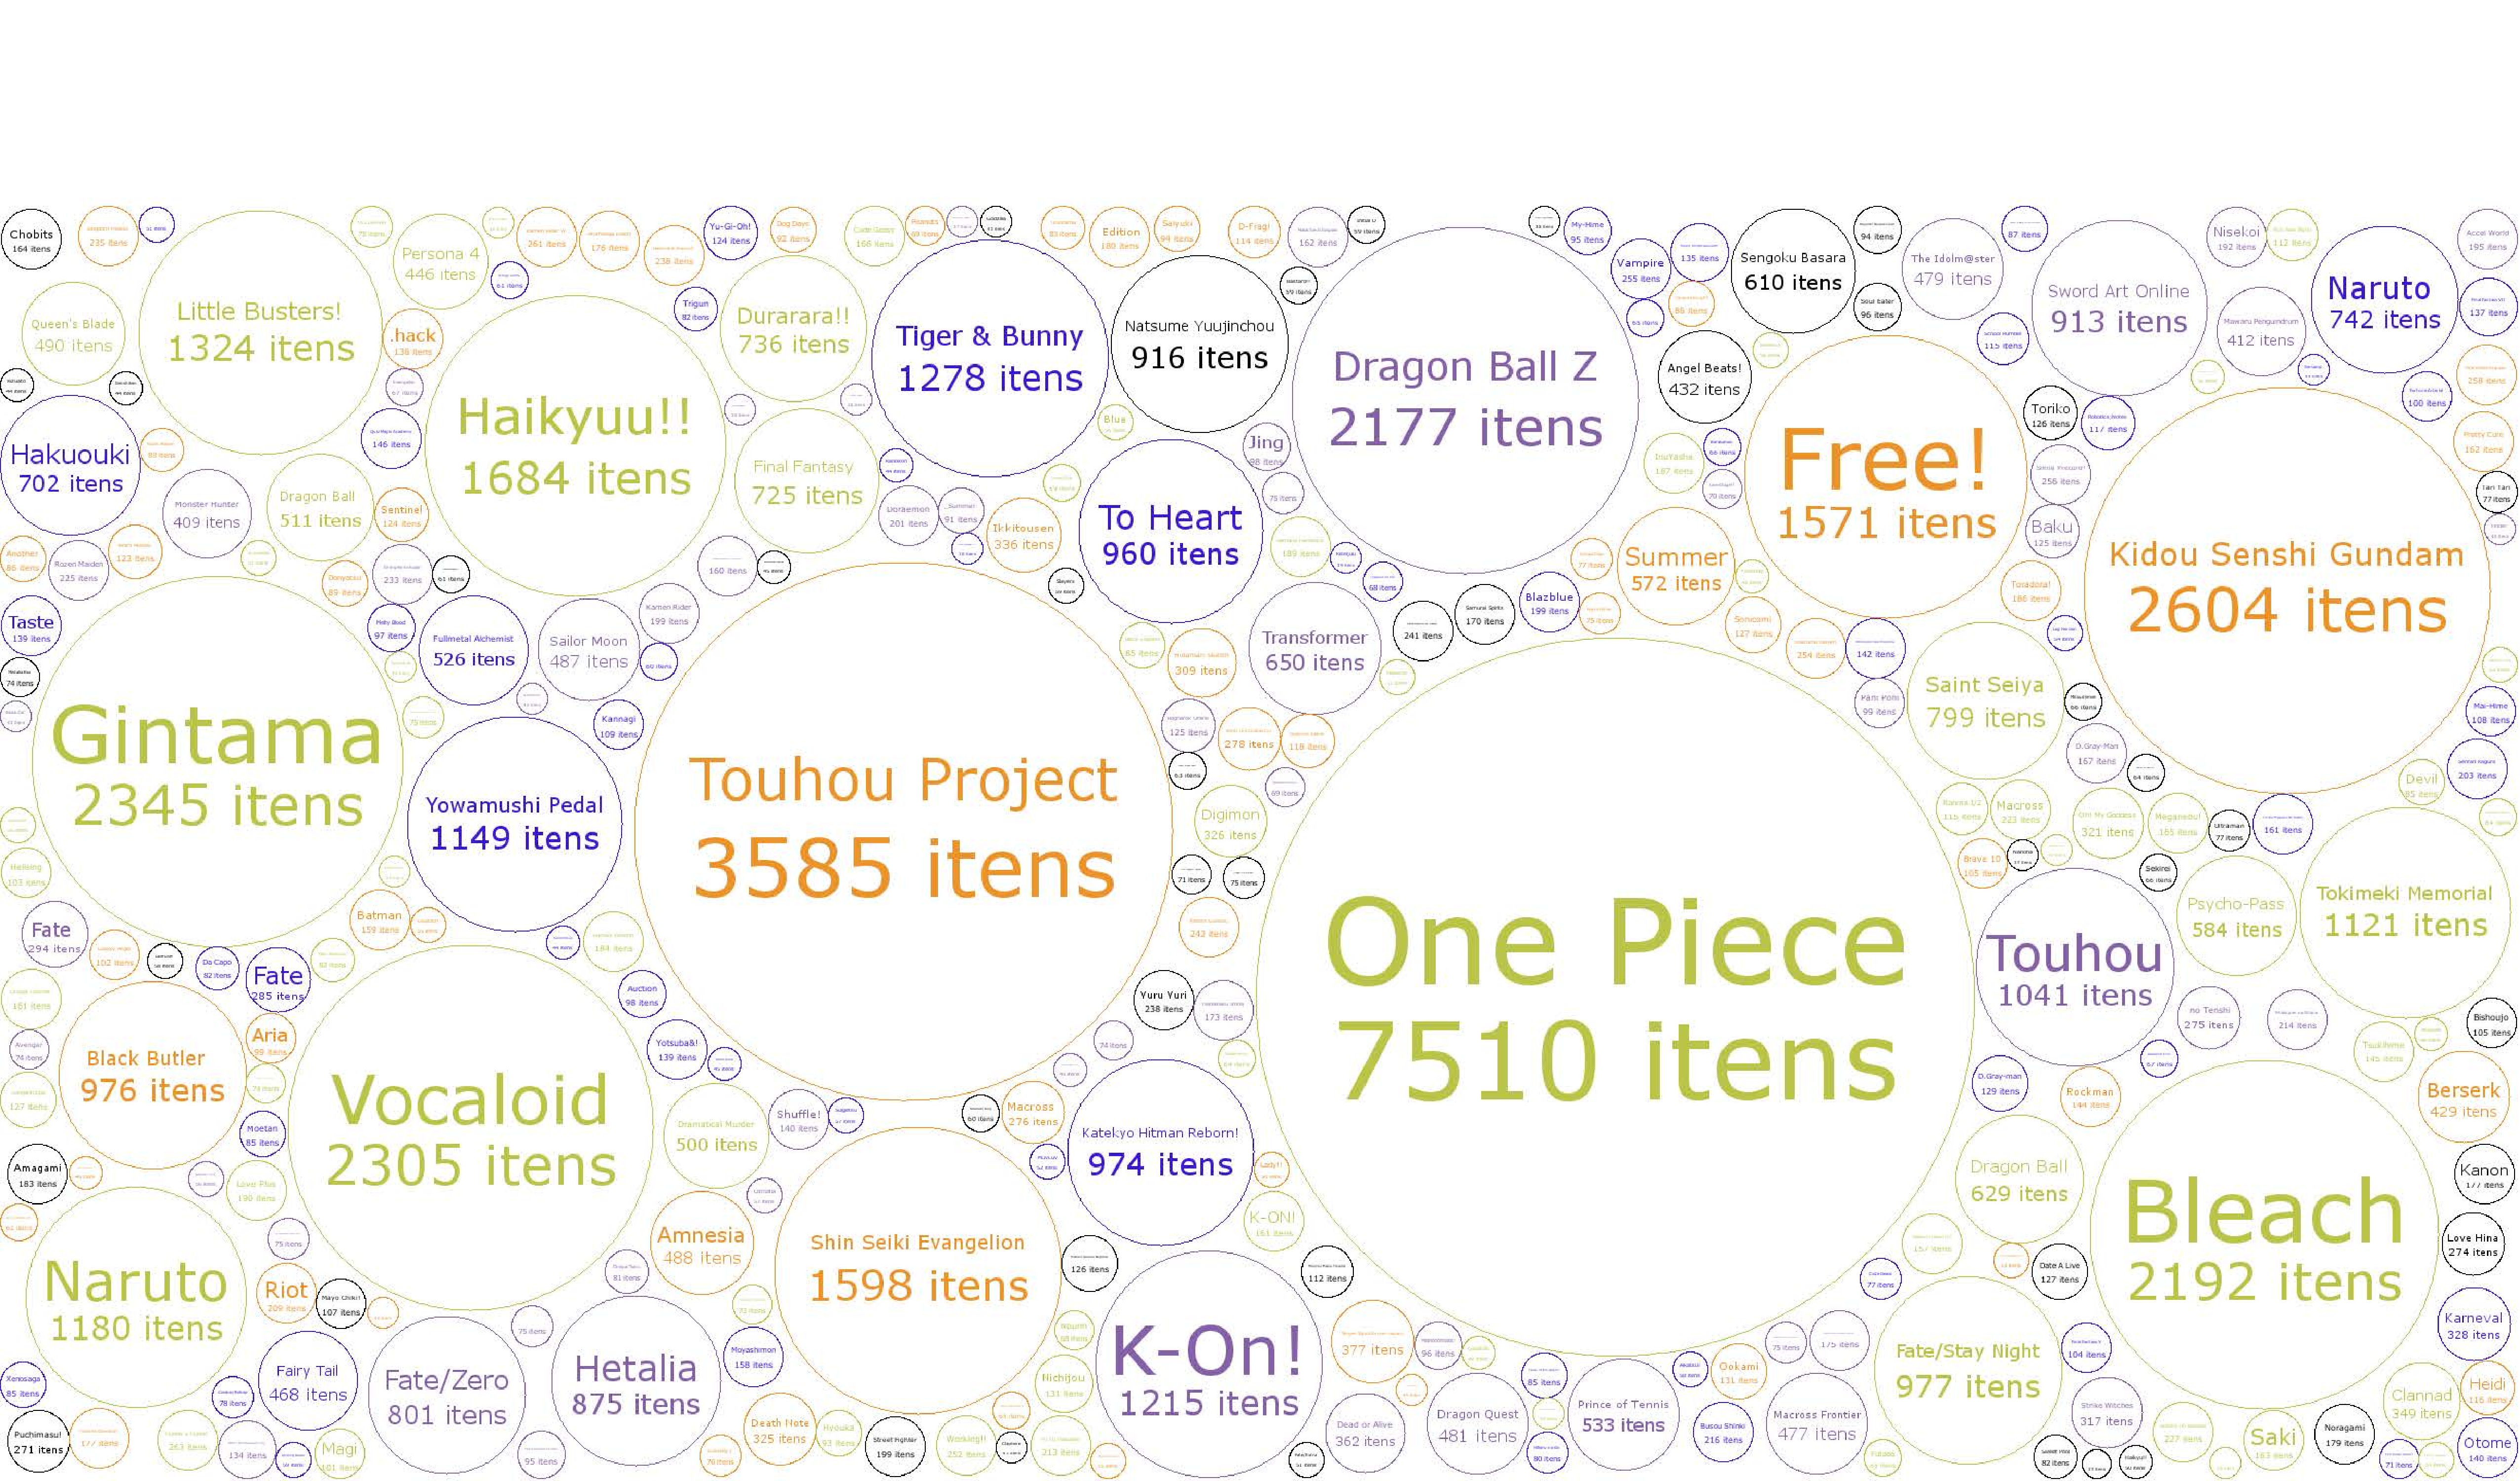
\includegraphics[width=0.5\linewidth]{collection_amount_bubbles.pdf} 
\includegraphics[width=0.5\linewidth]{writter.pdf}
             \caption{A esqueda representação da quantidade de itens por franquia. A direita representação das profissões com maior número de envolvidos na produção de itens da cultura popular japonesa.} \label{collaborator}
             \end{figure}
            \end{block}
            \vfill

            \begin{block}{Conclusão}
             Pode-se supor com as informações obtidas, que entre a imensa quantidade de produtos produzidos no Japão a maioria é de caráter literário devido a um alto nível de educação no país.
              
%%% References
            \end{block}
            \vfill
            \begin{block}{Referências Bibliográficas}
              \bibliographystyle{plain}
\begin{thebibliography}{2}

\bibitem{integral}
{P. Viola; M. Jones.}
\newblock {\emph{Rapid object detection using a boosted cascade of simple
features}. In IEEE Computer Vision and Pattern Recognition (pp. I:511–518), 2001.}

\bibitem{representation}
{Konstantinos G. Derpanis.}
\newblock {\emph{Integral image-based representations}, Department of Computer Science and Engineering, York University, New York, 2007.}

\bibitem{lang}
{Marco Lui; Timothy Baldwin.}
\newblock {\emph{langid.py: An Off-the-shelf Language Identification Tool}, Department of Computing and Information Systems, University of Melbourne, VIC 3010, Australia.}

\bibitem{tutorial} {Fredrik Lundh}.
\newblock {\emph{The Python Imaging Library Handbook}, 2014, disponível em \url{http://effbot.org/imagingbook/}}\\~\\
testet

te
t
e
t
\end{thebibliography}
            \end{block}
            \vfill}
          % ---------------------------------------------------------%
          % end the column
        \end{minipage}
      \end{beamercolorbox}
    \end{column}
    % ---------------------------------------------------------%
    % end the column
  \end{columns}
  \vskip1ex
\end{frame}
\end{document}


%%%%%%%%%%%%%%%%%%%%%%%%%%%%%%%%%%%%%%%%%%%%%%%%%%%%%%%%%%%%%%%%%%%%%%%%